\documentclass[a4paper, twocolumn]{article}
\usepackage[T1]{fontenc}
\usepackage[utf8]{inputenc}
%\usepackage[light,condensed,math]{kurier}
\usepackage[ngerman]{babel}
\usepackage{ntheorem}
\usepackage{graphicx}
\usepackage{floatrow}
\usepackage{float}
\usepackage{hyperref}
\usepackage{mathtools}
\usepackage{amssymb}
\usepackage{minted}
\usepackage{microtype}
\usepackage[all]{nowidow}
\usepackage{centernot}
\usepackage{listings}
\theoremstyle{break}

\lstset{
	basicstyle=\ttfamily,
	columns=fullflexible,
	frame=single,
	breaklines=true,
	postbreak=\mbox{\textcolor{red}{$\hookrightarrow$}\space},
}

\newtheorem{formula}{Formel}[section]
\newtheorem{defi}{Definition}[section]
\newtheorem{ann}{Bemerkung}[section]
\newtheorem{der}{Folgerung}[section]
\newtheorem{ex}{Beispiel}[section]
\newtheorem{why}{Vorteile}[section]
\newtheorem{whynot}{Nachteile}[section]

\title{Cheat Sheet: Programmierparadigmen}
\author{Adrian E. Lehmann}
\begin{document}
	\section{Lambda-Kalkül}
\subsection{Untypisiertes Lambdakalkül}
\textbf{linksassoziativ}
\begin{defi}[$\alpha$-Äquiv]
	Terme $t_1$,  $t_2$ $\alpha$-äquivalent $\Leftrightarrow$ $t_1$ durch Ersetzen der gebunden Variablen in $t_2$ überführbar
\end{defi}
Beispiel: $\lambda y.y \stackrel{\alpha}{=} \lambda x.x$

\subsubsection{Ausführungsreihenfolge}

\begin{defi}[Normalenreihenfolge]
	Linkest-äu\ss{}ersten Term zuerst
\end{defi}
Beispiel 1:\\
$$(\lambda x.x)((\lambda x.x) (\lambda z. (\lambda x.x) z))$$
$$ \Rightarrow ((\lambda x.x) (\lambda z. (\lambda x.x) z))$$
$$ \Rightarrow (\lambda z. (\lambda x.x) z)$$
$$ \Rightarrow (\lambda z. z)$$
Beispiel 2:\\
$$(\lambda y. (\lambda x. y (\lambda z.z) x)) ((\lambda x.x) (\lambda y.y))$$
$$\Rightarrow \lambda x. ((\lambda x1.x1) (\lambda y.y)) (\lambda z.z) x $$
$$\Rightarrow \lambda x. (\lambda y.y) (\lambda z.z) x$$
$$\Rightarrow \lambda x. (\lambda z.z) x $$
$$\Rightarrow \lambda x. x $$
\begin{defi}[Call-by-name]
		Linkest-äu\ss{}ersten Term zuerst, falls nicht von lambda umgeben
\end{defi}
Beispiel 1:\\
$$(\lambda x.x)((\lambda x.x) (\lambda z. (\lambda x.x) z))$$
$$ \Rightarrow ((\lambda x.x) (\lambda z. (\lambda x.x) z))$$
$$ \Rightarrow (\lambda z. (\lambda x.x) z)$$
Beispiel 2:\\
$$(\lambda y. (\lambda x. y (\lambda z.z) x)) ((\lambda x.x) (\lambda y.y))$$
$$\Rightarrow \lambda x. ((\lambda x_1.x_1) (\lambda y.y)) (\lambda z.z) x $$
\begin{defi}[Call-by-value]
	Linkest-äu\ss{}ersten Term zuerst, falls nicht von lambda umgeben und dessen Argument ein Wert ist
\end{defi}
Beispiel 1:\\
$$(\lambda x.x)((\lambda x.x) (\lambda z. (\lambda x.x) z))$$
$$ \Rightarrow ((\lambda x.x) (\lambda z. (\lambda x.x) z))$$
$$ \Rightarrow (\lambda z. (\lambda x.x) z)$$
Beispiel 2:\\
$$(\lambda y. (\lambda x. y (\lambda z.z) x)) ((\lambda x.x) (\lambda y.y))$$
$$\Rightarrow \lambda y. (\lambda x. y (\lambda z.z) x)) (\lambda y.y)$$
$$\Rightarrow \lambda x. (\lambda y.y) (\lambda z.z) x))$$

\subsubsection{Rekursion}
Parametrisiere rekursiven Aufruf als erstes Argument, verwende Y kombinator\\
Beispiel:\\
$$f = \lambda fak. \lambda n. \medspace (\text{isZero}\medspace n)  \medspace c_1 \medspace (\text{times} \medspace n \medspace (fak (\text{sub}\medspace n \medspace c_1)))$$
$$fak = Y \medspace f$$

\subsubsection{Church Zahlen}
\begin{align*}
c_0 &= \lambda s.\ \lambda\ z.\ z\\
c_1 &= \lambda s.\ \lambda\ z.\ s\ z\\
& \cdots \\
c_n &= \lambda s. \lambda z.\ s^n\ z\\
succ &= \lambda n. \lambda s. \lambda z.\ s\ (n\ s\ z)\\
plus &= \lambda m. \lambda n. \lambda s. \lambda z.\ m\ s\ (n\ s\ z)\\
times &= \lambda m. \lambda n. \lambda s.\ n\ (m\ s)\\
exp &= \lambda m. \lambda n.\ n\ m\\
\end{align*}


	\subsection{Typisierung}
\begin{center}
	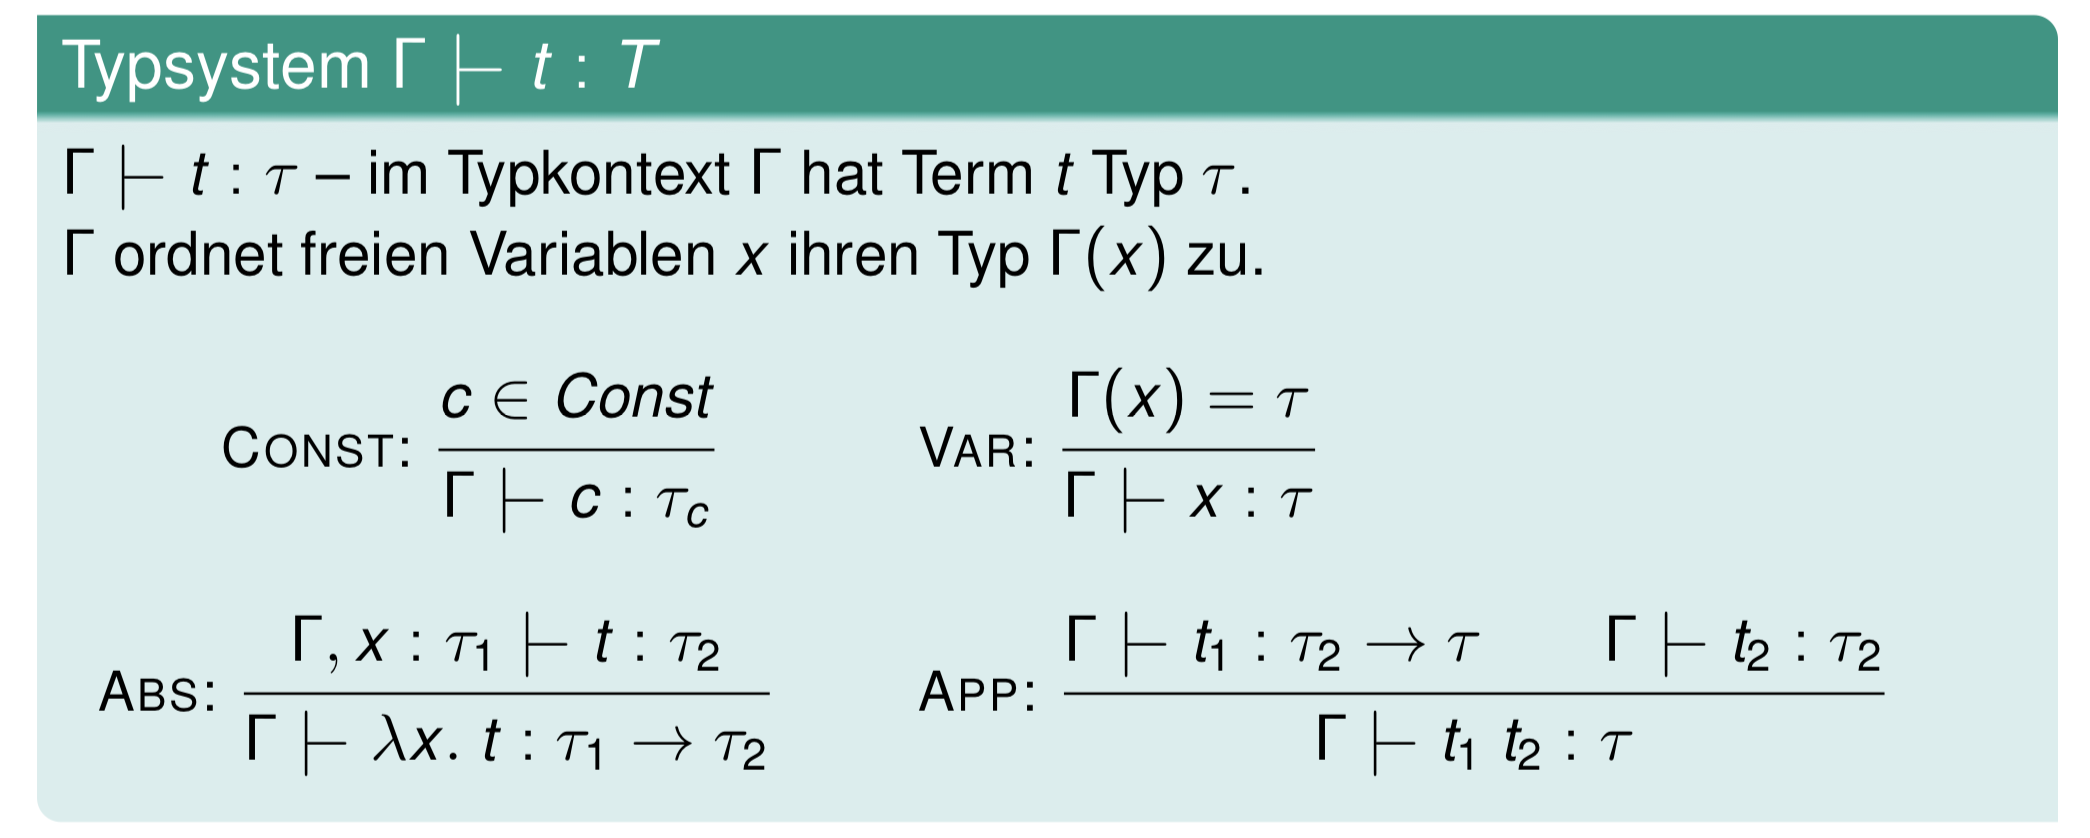
\includegraphics[width=0.75\textwidth]{images/types.png}	
\end{center}
\begin{center}
		
\includegraphics[width=0.75\textwidth]{images/let.png}
\end{center}
Beispiel:\\
\begin{center}
	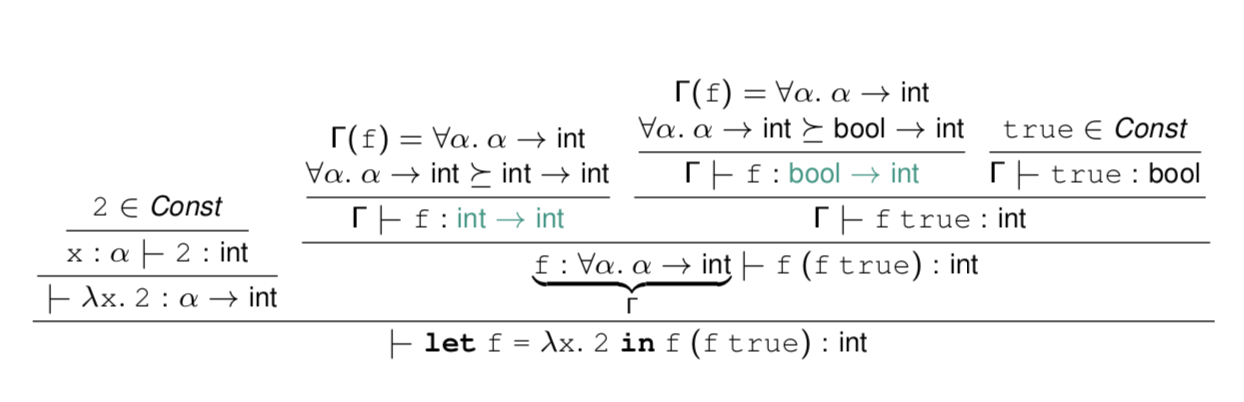
\includegraphics[width=0.75\textwidth]{images/let_ex.png}
\end{center}
\subsubsection{Typisierungsgleichungen}
$$APP \medspace\frac{\Gamma \vdash t_1 : \alpha_2 \medspace\medspace\medspace \Gamma \vdash t_2 : \alpha_3}{\Gamma \vdash t_1 \medspace t_2 : \alpha_1} \rightsquigarrow C_{new} = C \cup \{\alpha_2 = \alpha_3 -> \alpha_1\}$$

$$ABS \medspace\frac{\Gamma, x : \alpha_2 \vdash t : \alpha_3}{\Gamma \vdash \lambda x.t:\alpha_1} \rightsquigarrow C_{new} = C \cup \{\alpha_1 = \alpha_2 -> \alpha_3\}$$

$$VAR \medspace\frac{(x: \alpha_1)(x) = \alpha_2}{\Gamma \vdash x : \alpha_2} \rightsquigarrow C_{new} = C \cup \{\alpha_1 = \alpha_2\}$$

$$Const \medspace\frac{c \in Const}{\Gamma \vdash x : \alpha_1} \rightsquigarrow C_{new} = C \cup \{\alpha_1 = \alpha_c\}$$

\paragraph{Let}
Betrachte:
$$\frac{\Gamma \vdash t_1: \alpha_2 \medspace \Gamma' \vdash t_2: \alpha_3}{\Gamma \vdash \textbf{let} x = t_1 in t_2 : \alpha_1}$$

\begin{enumerate}
	\item Setze $C_0 \coloneqq \{ \alpha_1 = \alpha_3 \}$
	\item Bestimme $C_{let}$ (linker Teilbaum) und $\sigma_{C_{let}}$
	\item Sei $\Gamma_r$ Typannahme rechter Teilbaum, dann ist $\Gamma_r = \Gamma, x: \forall \alpha. ...$
	\item Bestimme $C_{let}' = \{\alpha_i = \sigma_{let}(\alpha_i)\}$
	\item Bestimme constraints rechter Teilbaum $C_r$
	\item Bestimme $\sigma_{(C_0 \cup C_r \cup C_{let}')}$
\end{enumerate}
	\section{MPI}

Boilerplate: 
\begin{minted}[breaklines]{C}
#include "mpi.h"
int main(int argc, char** argv) {
    int size, rank;
    MPI_Init(&argc, &argv);
    MPI_Comm_size(MPI_COMM_WORLD, size);
    MPI_Comm_rank(MPI_COMM_WORLD, rank);
    if(rank == 0) { /*... */ } else { /* ... */ } // Root node check
    MPI_Finanlize();
    return 0;
}
\end{minted}

\subsection{Functions}

\begin{minted}[breaklines]{C}
MPI_Barrier(MPI_Comm comm);

int MPI_Send(void* buffer, int count, MPI_Datatype datatype, int dest, int tag, MPI_Comm comm);

int MPI_Recv(void* buffer, int count, MPI_Datatype datatype, int source, int tag, MPI_Comm comm, MPI_Status* status);

int MPI_Bcast(void* buffer, int count, MPI_Datatype t, int root, MPI_Comm comm);

int MPI_Scatter(void* sendbuf, int sendcount, MPI_Datatype sendtype, void* recvbuf, int recvcount, MPI_Datatype recvtype, int root, MPI_Comm comm);

int MPI_Gather(void* sendbuf, int sendcount, MPI_Datatype sendtype, void* recvbuf, int recvcount, MPI_Datatype recvtype, int root, MPI_Comm comm);

int MPI_Allgather( void* sendbuf, int sendcount, MPI_Datatype sendtype, void* recvbuf, int recvcount, MPI_Datatype recvtype, MPI_Comm comm);

int MPI_Alltoall( void *sendbuf, int sendcount, MPI_Datatype sendtype, void *recvbuf, int recvcount, MPI_Datatype recvtype, MPI_Comm comm);

int MPI_Reduce(void* sendbuf, void* recvbuf, int count, MPI_Datatype type, MPI_Op op, int root, MPI_Comm comm);
\end{minted}
\begin{center}
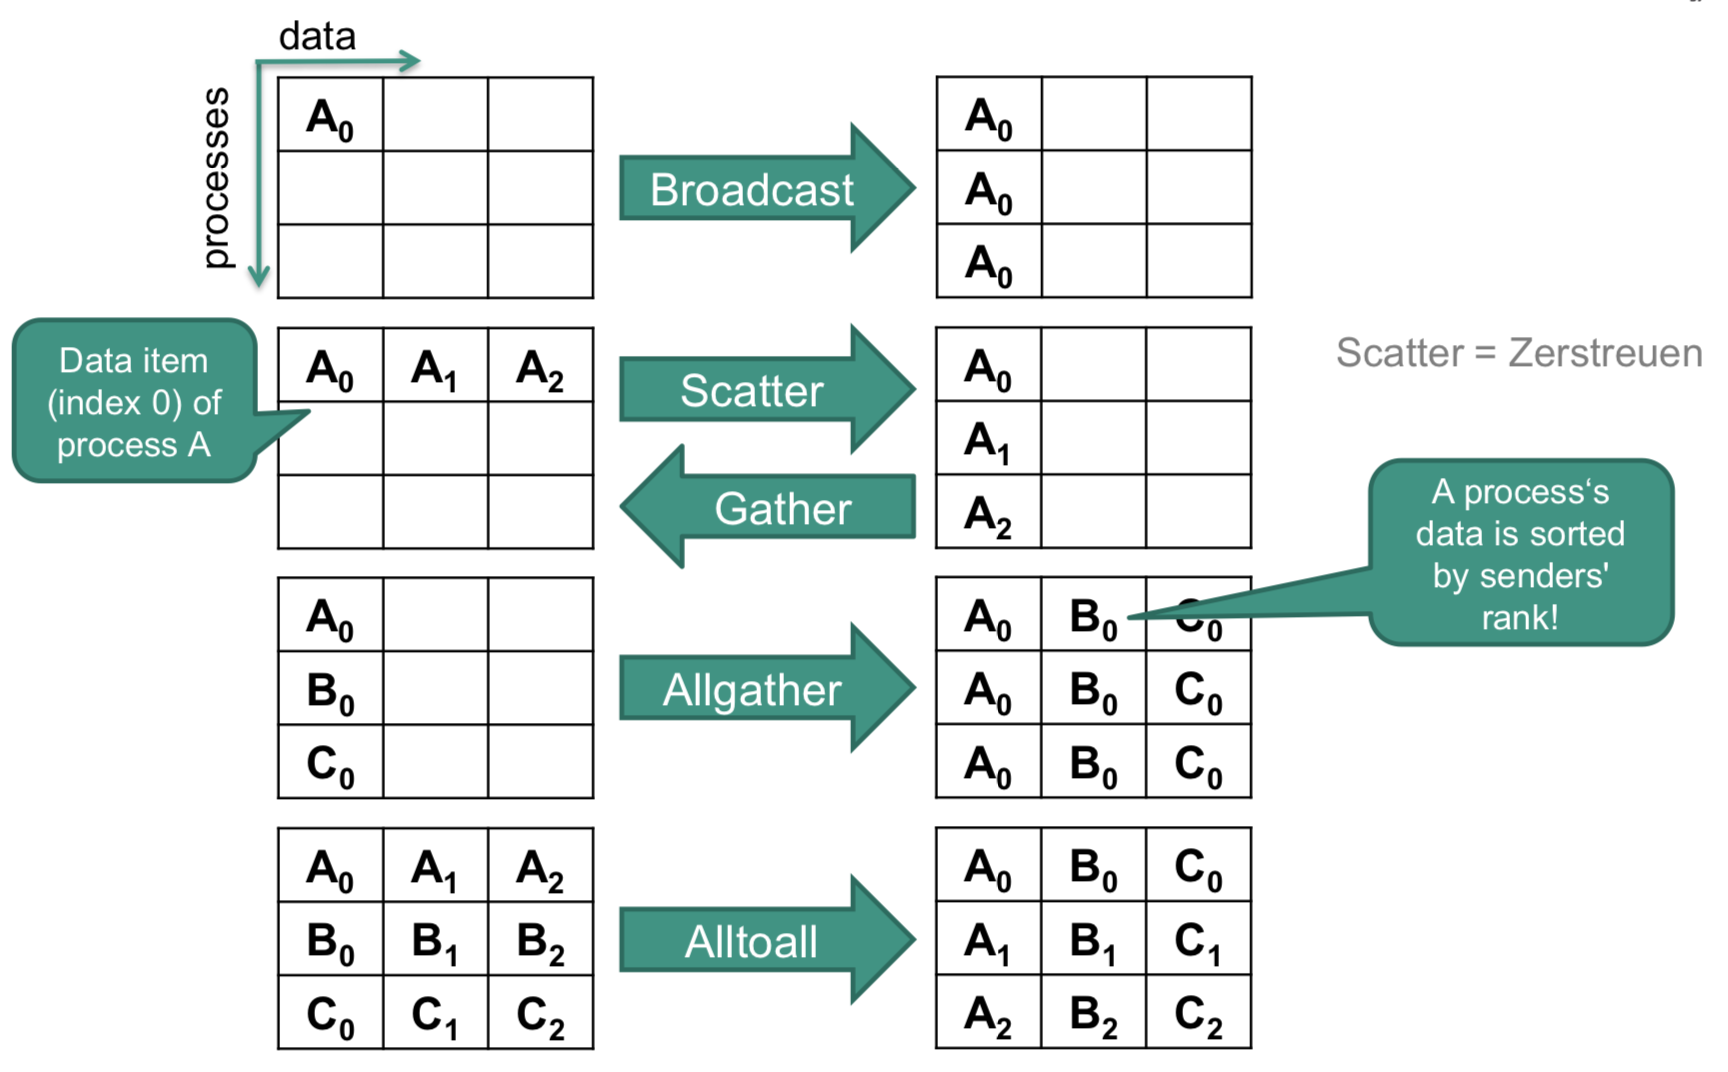
\includegraphics[width=\columnwidth]{images/MPI.png}
\end{center}
Example:
\begin{minted}[breaklines]{C}
if (myrank == 0) {
    strcpy(msg, "Hello student!");
    MPI_Send(msg, strlen(msg)+1, MPI_CHAR, 1, tag, MPI_COMM_WORLD);
} else {
    MPI_Recv(msg, 20, MPI_CHAR, 0, tag, MPI_COMM_WORLD, &status); 
    printf("received \"%s\"\n", msg);
}
\end{minted}
MPI-Datatypes: \texttt{MPI\_INT, MPI\_CHAR, MPI\_FLOAT,  MPI\_DOUBLE, ...}\\

\paragraph{Operations for \texttt{MPI\_Reduce}}
Mathematical Operations : \texttt{MPI\_MAX , MPI\_MIN , MPI\_SUM , MPI\_PROD} \\
Boolean Operations (logical and bitwise): \texttt{MPI\_LAND , MPI\_BAND , MPI\_LOR , MPI\_BOR, ...}\\

\subsection{Modes}

Blocking (default) vs. non-blocking\\

\textbf{Send-modes:}\\
\begin{enumerate}
	\item Synchronous: No buffer, synchronization (both sides wait for each other)
	\item Buffered:	Explicit buffering, no synchronization (no wait for each other)
	\item Ready: No buffer, no synchronization, matching receive must already be initiated
	\item Standard: May buffer or not, can be synchronous (implementation dependent)
\end{enumerate}





	\section{Parallelism}
Speedup:
$$S(n) = \frac{T(1)}{T(n)}$$
Ahmdahl's law:
$$ S(n) = \frac{1}{(1 - p)+\frac{p}{n}}$$
wobei $p$ der parallelisierbare Anteil ist (in \%)
\subsection{Deadlocks}
\paragraph{Coffman conditions}
\begin{enumerate}
	\item Mutual Exclusion
	\item Hold and wait
	\item No preemption
	\item Circular wait
\end{enumerate}
All of these conditions must apply for a deadlock to be possible
\subsection{Livelocks}
Threads switching but not making any progress
\subsection{Stravation}
Occurs if a thread cannot aquire any resources even if no deadlocks exist

\subsection{Flynn's taxonomy}

\begin{enumerate}
	\item SISD: Single instruction x single data
	\item SIMD: Single instruction x multiple data
	\item MIMD: Multiple instruction x multiple data	
	\item MISD: Multiple instruction x multiple data
\end{enumerate}
	\section{Design by contract}
\subsection{JML}

\texttt{@requires} und \texttt{@ensures} als Syntax für Vor- und Nachbedingung\\
Syntax:
\begin{itemize}
  \item $a ==> b$: a implziert b
  \item $a <==> b$: a gdw. b
  \item $a <=!=> b$: a gdw. nicht b
  \item $\backslash result$: Return wert
  \item $\backslash old(E)$: Wert von E im Status vor der Methodenausführung
\end{itemize}
Auch möglich $\backslash forall$ oder $\backslash exists$ zu verwenden.\\

Methoden können als $@pure$ annotiert werden.

\subsection{Liskov Substitution Principle}
Overriding methods must ensure:\\
\textbf{Precondition cannot be stronger} and \textbf{Postcondition cannot be weaker}\\

	\section{Compiler}
\subsection{Grammar Engineering}
\subsubsection{First sets}
$First(X)$ bestimmen:
\begin{enumerate}
	\item Falls $X$ Terminal: $First(X) = \{X\}$
	\item Falls $X  \rightarrow \epsilon$ füge $\epsilon$ zu $First(X)$
	\item Falls $X \rightarrow Y_1..Y_n$ füge $First(Y_1..Y_n)$ zu $First(X)$
	\item $First(Y_1..Y_n)$ ist entweder
	\begin{enumerate}
		\item $First(Y_1)$, iff $Y_1  \nrightarrow \epsilon$
		\item $First(Y_1) \backslash \{\epsilon\} \cup First(Y_2..Y_n)$,  falls $\exists k \in [2,n]: Y_k \nrightarrow \epsilon$
		\item rekursiv fortführen
	\end{enumerate}
\end{enumerate}
\subsubsection{Follow sets}
$Follow(X)$ bestimmen:
\begin{enumerate}
	\item Füge $\#$ zu $Follow(X)$, falls $X=S$
	\item Falls $A \rightarrow aXb$ und $\epsilon \centernot\in First(b)$, dann füge $First(b)$ zu $Follow(X)$
	\item Falls $A \rightarrow aX$, dann füge $Follow(A)$ zu $Follow(X)$
	\item Falls $A \rightarrow aXb$ und $\epsilon \in First(b)$, dann füge $First(b) \cup Follow(A)$ zu $Follow(X)$, 
\end{enumerate} 
\subsubsection{SLL(k)-Kriterium}
Eine (kontextfreie) Grammatik ist genau dann eine SLL(k)-Grammatik, wenn für alle Paare von Produktionen
\(A \rightarrow \alpha|\beta, \alpha \neq \beta\), gilt:
\[\mathit{First}_k(\alpha\mathit{Follow}_k(A)) \cap \mathit{First}_k(\beta\mathit{Follow}_k(A)) = \varnothing\]

\subsubsection{SLL(1)-Kriterium}
\textbf{Für alle Produktionen $A \rightarrow \alpha \mid \beta$:}\\
Falls $\alpha \nRightarrow^{*} \epsilon$ und $\beta \nRightarrow^{*} \epsilon$, so muss gelten:
$$First(\alpha) \cap First(\beta) = \emptyset$$
Falls $\alpha \nRightarrow^{*} \epsilon$, so zusätzlich gelten:
$$Follow(A) \cap First(\beta) = \emptyset$$
\subsection{Abstrakte Syntax}
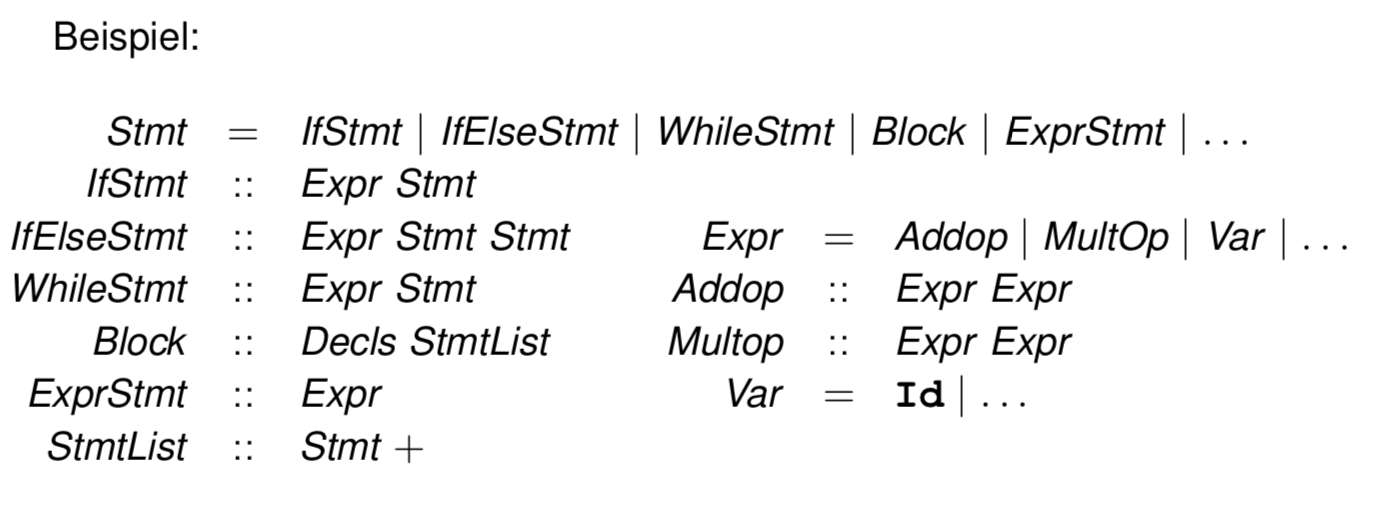
\includegraphics[width=\columnwidth]{images/abstract_syntax.png}
	\clearpage
	\section{Appendices}
	% !TeX root = ../propa-cheat-sheet.tex
\section{Haskell Prelude functions}
\subsection{Collections}
\begin{minted}[breaklines]{haskell}
elem :: Eq a => a -> t a -> Bool 
maximum :: forall a. Ord a => t a -> a
minimum :: forall a. Ord a => t a -> a
sum :: Num a => t a -> a
\end{minted}
\subsubsection{Lists}
\begin{minted}[breaklines]{haskell}
map :: (a -> b) -> [a] -> [b]
(++) :: [a] -> [a] -> [a] -- Concat lists
filter :: (a -> Bool) -> [a] -> [a]
head :: [a] -> a -- first element
last :: [a] -> a -- last element
tail :: [a] -> [a] -- everything except the first element
init :: [a] -> [a] -- everything except the last element
null :: Foldable t => t a -> Bool -- Empty check
length :: Foldable t => t a -> Int
reverse :: [a] -> [a]
(!!) :: [a] -> Int -> a -- Index operator
any :: Foldable t => (a -> Bool) -> t a -> Bool -- Test wether any element satisfies a predicate
all :: Foldable t => (a -> Bool) -> t a -> Bool -- Test wether all elements satisfies a predicate
replicate :: Int -> a -> [a] -- replicate n x is a list of length n with x the value of every element.
\end{minted}
\subsubsection{Infinite lists}
\begin{minted}[breaklines]{haskell}
iterate :: (a -> a) -> a -> [a] -- iterate f x == [x, f x, f (f x), ...]
repeat :: a -> [a] -- infinite list from first element: repeat x = [x, x, ...]
cycle :: [a] -> [a] -- turn finite list into circular infinite list
\end{minted}
\subsubsection{Sub-Lists}
\begin{minted}[breaklines]{haskell}
take :: Int -> [a] -> [a]
drop :: Int -> [a] -> [a]
splitAt :: Int -> [a] -> ([a], [a])
takeWhile :: (a -> Bool) -> [a] -> [a]
dropWhile :: (a -> Bool) -> [a] -> [a]
span :: (a -> Bool) -> [a] -> ([a], [a]) -- Tuple longest list of elements satisfying p and second element remainder
break :: (a -> Bool) -> [a] -> ([a], [a]) -- inverse of span, applied to a predicate p and a list xs, returns a tuple where first element is longest prefix (possibly empty) of xs of elements that do not satisfy p and second element is the remainder of the list
zipWith :: (a -> b -> c) -> [a] -> [b] -> [c]
zip = zipWith (,)
unzip :: [(a, b)] -> ([a], [b])
\end{minted}
\subsubsection{Folding}

\textbf{Right to left:}
\begin{minted}[breaklines]{haskell}
foldr :: (a -> b -> b) -> b -> t a -> b
\end{minted}
Usage:
\begin{minted}[breaklines]{haskell}
folded = foldr (\val -> \acc -> newAcc) acc coll
\end{minted}
\textbf{Left to right:} 
\begin{minted}[breaklines]{haskell}
foldl :: (b -> a -> b) -> b -> t a -> b
\end{minted}
Usage:
\begin{minted}[breaklines]{haskell}
folded = foldl (\acc -> \val -> newAcc) acc coll
\end{minted}
\textbf{Bsp.:}
\begin{minted}[breaklines]{haskell}
foldr (+) 0 [1,2,3,4]
\end{minted}
berechnet den Wert (1+(2+(3+(4+0)))) – rechts-geklammert 
\begin{minted}[breaklines]{haskell}
foldl (+) 0 [1,2,3,4]
\end{minted}
den Wert ((((0+1)+2)+3)+4) – links-geklammert\\
\subsubsection{Tuples}
\begin{minted}[breaklines]{haskell}
fst :: (a,b) -> a
snd :: (a,b) -> b
curry :: ((a, b) -> c) -> a -> b -> c
uncurry :: (a -> b -> c) -> (a, b) -> c
\end{minted}
\subsection{Values and numbers}
\begin{minted}[breaklines]{haskell}
succ :: a -> a
pred :: a -> a
even :: Integral a => a -> Bool
odd :: Integral a => a -> Bool
gcd :: Integral a => a -> a -> a
lcm :: Integral a => a -> a -> a
(^) :: (Num a, Integral b) => a -> b -> a 
\end{minted}
\subsubsection{Float}
\begin{minted}[breaklines]{haskell}
isNaN :: a -> Bool
isInfinite :: a -> Bool
\end{minted}
\subsection{Misc}
\subsubsection{IO}
\begin{minted}[breaklines]{haskell}
putStrLn :: String -> IO ()
print :: Show a => a -> IO ()
getLine :: IO String
getChar :: IO Char
\end{minted}
\subsubsection{Maybe}
\begin{minted}[breaklines]{haskell}
data Maybe = Nothing |  Just a
\end{minted}
\begin{minted}[breaklines]{haskell}
maybe :: b -> (a -> b) -> Maybe a -> b
\end{minted}
Usage:
\begin{minted}[breaklines]{haskell}
value = maybe orElse mappingAToB maybe instance
\end{minted}

	\newpage
	\appendix\section{Useful prolog functions}
\subsection{Types}
\begin{minted}[breaklines]{prolog}
atom(X) /** Wahr falls Term ein Atom **/
integer(X) /** Wahr falls Integer **/
var(X) /** Wahr falls freie Variable **/
\end{minted}
\subsection{Listen}
\begin{minted}[breaklines]{prolog}
member(X,L) /** is X in L **/
append(S1,S2,S) /** S1 ++ S2 == S **/
rev(X,Y) /** reverse **/
permute(P,X) /** permutations of P **/
\end{minted}
\subsection{Arithmetic}
\begin{minted}[breaklines]{prolog}
X is 3*A+4 /** nicht rückwärts ausführbar! **/
between(Low,High,Value) /** Integers between limits **/  
\end{minted}
	\newpage
	% !TeX root = ../propa-cheat-sheet.tex
\appendix\section{Java Reference}
\paragraph{\texttt{java.util.Thread}}
\begin{minted}[breaklines]{java}
void Thread#run()
boolean Thread#isInterrupted()
void Thread#interrupt()
boolean Thread#isAlive()
void Thread#sleep(int)
void Thread#join()
\end{minted}
\paragraph{\texttt{volatile}}
\begin{minted}[breaklines]{java}
class A {
    volatile Type name; // prevent caching and reordering around usages
}
\end{minted}
\paragraph{\texttt{AtomicInteger}}
\begin{minted}[breaklines]{java}
AtomicInteger(int)
int AtomicInteger#get()
int AtomicInteger#incrementAndGet()
int AtomicInteger#decrementAndGet()
boolean AtomicInteger#compareAndSet(int, int) // first parameter oldVal, second parameter sndVal; replaces iff atomic integer has value oldVal
\end{minted}
\paragraph{\texttt{Locks}}
\begin{minted}[breaklines]{java}
void Lock#lock()
void Lock#unlock()
boolean Lock#tryLock() // only take lock if it's avb
\end{minted}
Implementation of interface: \texttt{ReentrantLock}
\begin{minted}[breaklines]{java}
ReentrantLock​(boolean) // Constructor with fair option
\end{minted}
\paragraph{\texttt{Semaphore}}
Allows n threads into a critical section
\begin{minted}[breaklines]{java}
Semaphore(int, boolean) // Constructor with amoint and fair option
void Semaphore#aquire()
void Semaphore#release()
boolean Semaphore#tryAquire()
\end{minted}
\paragraph{\texttt{CyclicBarrier}}
\begin{minted}[breaklines]{java}
CyclicBarrier(int)
void CyclicBarrier#await() // once called n times, all threads resume
\end{minted}
\paragraph{\texttt{CountDownLatch}}
Just like cyclic barrier only non-reusable: After n calls of \texttt{await} let's all threads through

\paragraph{\texttt{ExecutorServices}}
\begin{minted}[breaklines]{java}
Executors.newSingleThreadExecutor()
Executors.newFixedThreadPool(int)
Executors.newCachedThreadPool()
\end{minted}
Example:
\begin{minted}[breaklines]{java}
ExecutorService executor = Executors.newSingleThreadExecutor(); executor.execute(() -> {
    String threadName = Thread.currentThread().getName(); System.out.println("Hello " + threadName);
});

try {
    executor.shutdown();
    executor.awaitTermination(5, TimeUnit.SECONDS);
} catch(InterruptedException ex) { } finally {
     if (!executor.isTerminated()) {
          executor.shutdownNow();
     } 
}
\end{minted}
\paragraph{\texttt{Futures}}
\begin{minted}[breaklines]{java}
<T> Future<T>#submit(Callable<T> callable)
\end{minted}
 
\begin{minted}[breaklines]{java}
ExecutorService executorService = Executors.newCachedThreadPool(); 
List<Future<Integer>> futures = new ArrayList<Future<Integer>>(); 
for (int i = 0; i < 10; i++) {
    final int currentValue = i;
    futures.add(executorService.submit(() -> { return currentValue; }));
}
for (Future<Integer> future : futures) { 
    try {
         Integer result = future.get();
         System.out.println(result);
    } catch (ExecutionException ex) {}
} 
executorService.shutdown();
\end{minted}

\paragraph{\texttt{Completeable Future}}
\begin{minted}[breaklines]{java}
CompletableFuture<Integer> futureCount = CompletableFuture.supplyAsync( () -> {
    try {
         // simulate long running task 
         Thread.sleep(5000);
    } catch (InterruptedException ex) { }
    return 20; 
    }
);
CompletableFuture<String> modified = futureCount.thenApply((Integer count) -> {
     int transformedValue = count * 10;
     return transformedValue; 
     }
).thenApply(transformed -> "Finally create a string: " + transformed);
System.out.println(modified.get());
\end{minted}


\paragraph{\texttt{BlockingQueue}}
\begin{minted}[breaklines]{java}
T BlockingQueue<T>#take()
BlockingQueue<T>#put(T)
\end{minted}
Concrete impls:
\begin{itemize}
	\item LinkedBlockingQueue - unlimited
	\item ArrayBlockingQueue - limited
	\item PriorityBlockingQueue - sorted
\end{itemize}

\paragraph{\texttt{ForkJoin}}
\begin{minted}[breaklines]{java}
ForkJoinPool fjPool = new ForkJoinPool();
MyTask myTask = new MyTask(...);
fjPool.invoke(myTask);
\end{minted}
\begin{minted}[breaklines]{java}
public class MyTask extends RecursiveTask<Integer> {
@Override
public static Integer compute() {
// calculate something and return if problem small
MyTask leftTask = new MyTask(...); 
MyTask rightTask = new MyTask(...);
leftTask.fork();
rightTask.compute();
leftTask.join();
}
\end{minted}

	\newpage
	\appendix\section{Java  ByteCode}
Beispiele:\\
\textbf{Basic:}
\begin{minted}[breaklines]{java}
void calc(int x, int y) {
    int z = 4;
    x = y * z + x; 
}
\end{minted}
\begin{lstlisting}[language=JVMIS]
// Lade Konstante 4
iconst_4
// Schreibe in z
istore_3
// Lade y
iload_2
// Lade z
iload_3
// y * z
imul
// Lade x 
iload_1
// (y * z) + x 
iadd
// Speichere x
istore_1
\end{lstlisting}
\noindent\rule{\columnwidth}{0.4pt}
\textbf{If:}
\begin{minted}[breaklines]{java}
if(x==4) { A } else { B }
\end{minted}
\begin{lstlisting}[language=JVMIS]
    iload 0 // x laden
    bipush 4
    if_icmpeq label0 // falls gleich springe zu label0 
    goto label1 // springe zu label1
label0:
    A // then−Teil
    goto label2 
label1:
    B // else−Teil
    goto label2 
label2:
    // weitere Befehle
\end{lstlisting}
\noindent\rule{\columnwidth}{0.4pt}
\textbf{While:}
\begin{minted}[breaklines]{java}
while (x<10) { A }
\end{minted}
\begin{lstlisting}[language=JVMIS]
loopheader:
    iload 0 // x laden
    bipush 10
    if_icmplt loopbody // falls kleiner springe zu loopbody 
    goto afterloop // springe zu afterloop
loopbody:
    A // Schleifenkoerper
    goto loopheader // springe zu loopheader (naechste Iteration) 
afterloop:
    // weitere Befehle
\end{lstlisting}
\noindent\rule{\columnwidth}{0.4pt}
\textbf{Call:}\\
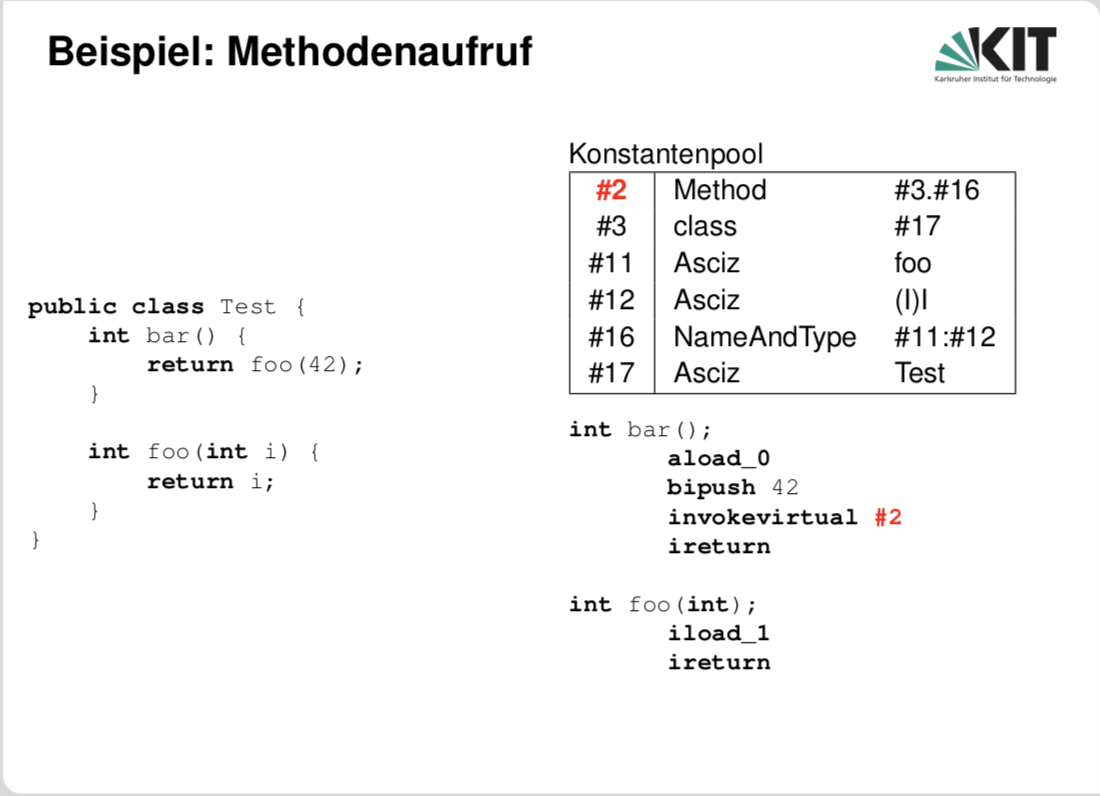
\includegraphics[width=\columnwidth]{images/byte_code_call.png}
\textbf{Conditional jumps:}
\begin{lstlisting}[language=JVMIS]
if_icmpeq target // Jump if equal
if_icmpne target // Jump if NOT equal
if_icmpge target // Jump if equal or greater than
if_icmpgt target // Jump greater than
if_icmple target // Jump if equal or less than
if_icmplt target // Jump if less than
\end{lstlisting}
\textbf{Misc:}
\begin{lstlisting}[language=JVMIS]
iinc x, y // increment variable x by y
aload_0 // load this ptr
putfield x // this.x = acc
\end{lstlisting}

\end{document}
